\chapter{Psalm 77}

\begin{figure}
  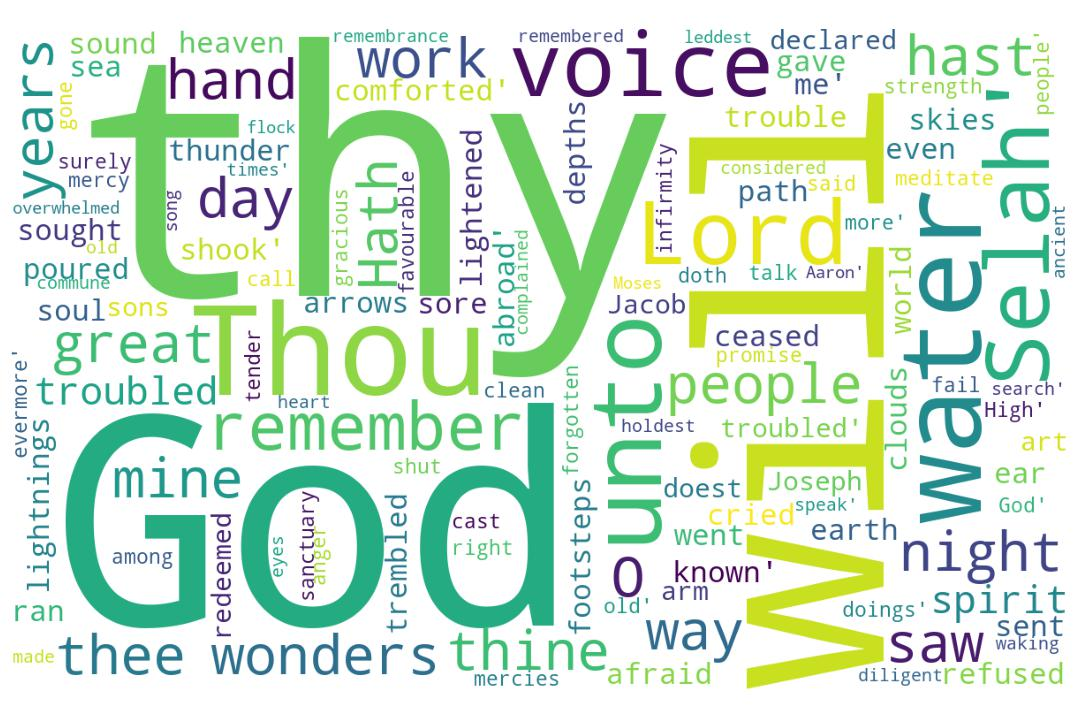
\includegraphics[width=\linewidth]{19OT-Psalms/Psalm77-WordCloud.jpg}
  \caption{Psalm 77 Word Cloud}
  \label{fig:Psalm 77 Word Cloud}
\end{figure}

\marginpar{\scriptsize \centering \fcolorbox{bone}{lime}{\textbf{GOD IS $\hdots$}}\\ (Psalm 77) \begin{compactenum}[I.][8]
    \item \textbf{My Silence} \index[scripture]{Psalms!Psa 077:04}(Psa 77:4)
    \item \textbf{My Searching} \index[scripture]{Psalms!Psa 077:06}(Psa 77:6)
    \item \textbf{My Song} \index[scripture]{Psalms!Psa 077:06}(Psa 77:6)
    \item \textbf{My Spech} \index[scripture]{Psalms!Psa 077:12}(Psa 77:12)
    \item \textbf{My Strength} \index[scripture]{Psalms!Psa 077:14}(Psa 77:14)
    \item \textbf{My Salvation} \index[scripture]{Psalms!Psa 077:15}(Psa 77:15)
    \item \textbf{My Saviour} \index[scripture]{Psalms!Psa 077:20}(Psa 77:20)
\end{compactenum}}
    

\marginpar{\scriptsize \centering \fcolorbox{bone}{yellow}{\textbf{A CHANGE OF}}\\
\fcolorbox{bone}{yellow}{\textbf{HEART AND MIND}}\\ (Psalm 77) 
\begin{compactenum}[I.][8]
    \item \textbf{There is Complaining} \index[scripture]{Psalms!Psa 077:03}(Psa 77:3)
    \item \textbf{There is Considering} \index[scripture]{Psalms!Psa 077:05}(Psa 77:5)
    \item \textbf{There is Communing with your Heart} \index[scripture]{Psalms!Psa 077:06}(Psa 77:6)
    \item \textbf{Thinking God Could Cast off his People} \index[scripture]{Psalms!Psa 077:07}(Psa 77:7)
    \item \textbf{But then Calling to Mind (remembering)} \index[scripture]{Psalms!Psa 077:11}(Psa 77:11)
    \item \textbf{And then God Confounds us} \index[scripture]{Psalms!Psa 077:13}(Psa 77:13) with his greatness, goodness, grace ...
    \item \textbf{That we can barely Contemplate Him} \index[scripture]{Psalms!Psa 077:14}(Psa 77:14)
\end{compactenum}}

\marginpar{\scriptsize \centering \fcolorbox{bone}{black}{\textbf{\textcolor{white}{THE PATH TO}}}\\ \fcolorbox{bone}{black}{\textbf{\textcolor{white}{DELIVERANCE}}}\\(Psalm 77) \begin{compactenum}[I.][8]
    \item \textbf{Revulsion} \index[scripture]{Psalms!Psa 077:02}(Psa 77:2)
    \item \textbf{Refusal} \index[scripture]{Psalms!Psa 077:03}(Psa 77:3)
    \item \textbf{Remembering} \index[scripture]{Psalms!Psa 077:03}\index[scripture]{Psalms!Psa 077:06}\index[scripture]{Psalms!Psa 077:11}\index[scripture]{Psalms!Psa 077:06}(Psa 77:3, 6, 10, 11)
    \item \textbf{Result} \index[scripture]{Psalms!Psa 077:10}(Psa 77:10)
    \item \textbf{Realization} \index[scripture]{Psalms!Psa 077:10}\index[scripture]{Psalms!Psa 077:13}(Psa 77:10, 13)
    \item \textbf{Redemption} \index[scripture]{Psalms!Psa 077:15}(Psa 77:15)
    \item \textbf{Revelation} \index[scripture]{Psalms!Psa 077:18}(Psa 77:18)
    \item \textbf{Rescue} \index[scripture]{Psalms!Psa 077:20}(Psa 77:20)
\end{compactenum}}


% \textcolor[cmyk]{0.99998,1,0,0}{
\footnote{\textcolor[rgb]{0.00,0.25,0.00}{\hyperlink{TOC}{Return to end of Table of Contents.}}}\footnote{\href{https://audiobible.com/bible/psalms_77.html}{\textcolor[cmyk]{0.99998,1,0,0}{Psalm 77 Audio}}}\textcolor[cmyk]{0.99998,1,0,0}{To the chief Musician, to Jeduthun, A Psalm of Asaph.}\\
\\
\textcolor[cmyk]{0.99998,1,0,0}{\fcolorbox{bone}{bone}{I} cried unto God with my voice, \emph{even} unto God with my voice; and he gave ear unto me.}
[2] \textcolor[cmyk]{0.99998,1,0,0}{In the day of my trouble \fcolorbox{bone}{bone}{I} sought the Lord: my sore ran in the night, and ceased not: my soul refused to be comforted.}\footnote{\textbf{Psalm 38:7} - For my loins are filled with a loathsome disease: and there is no soundness in my flesh.}
[3] \textcolor[cmyk]{0.99998,1,0,0}{\fcolorbox{bone}{bone}{I} remembered God, and was troubled: \fcolorbox{bone}{bone}{I} complained, and my spirit was overwhelmed. \fcolorbox{bone}{red}{\textcolor{white}{Selah}}.}
[4] \textcolor[cmyk]{0.99998,1,0,0}{Thou holdest mine eyes waking: \fcolorbox{bone}{bone}{I} am so troubled that \fcolorbox{bone}{bone}{I} cannot speak.}
[5] \textcolor[cmyk]{0.99998,1,0,0}{\fcolorbox{bone}{bone}{I} have considered the days of old, the years of ancient times.}\footnote{\textbf{Isaiah 46:10} - Declaring the end from the beginning, and from ancient times the things that are not yet done, saying, My counsel shall stand, and I will do all my pleasure:}
[6] \textcolor[cmyk]{0.99998,1,0,0}{\fcolorbox{bone}{bone}{I} call to remembrance my song in the night: \fcolorbox{bone}{bone}{I} commune with mine own heart: and my spirit made diligent search.}
[7] \textcolor[cmyk]{0.99998,1,0,0}{Will the Lord cast off for ever? and will he be favourable no more?}
[8] \textcolor[cmyk]{0.99998,1,0,0}{Is his mercy clean gone for ever? doth \emph{his} promise fail for evermore?}\footnote{\textbf{1 Kings 8:56} - Blessed be the LORD, that hath given rest unto his people Israel, according to all that he promised: there hath not failed one word of all his good promise, which he promised by the hand of Moses his servant.}
[9] \textcolor[cmyk]{0.99998,1,0,0}{Hath God forgotten to be gracious? hath he in anger shut up his tender mercies? \fcolorbox{bone}{red}{\textcolor{white}{Selah}}.}
[10] \textcolor[cmyk]{0.99998,1,0,0}{And \fcolorbox{bone}{bone}{I} said, This \emph{is} my infirmity: \emph{but} \emph{I} \emph{will} \emph{remember} the years of the right hand of the most High.}
[11] \textcolor[cmyk]{0.99998,1,0,0}{\fcolorbox{bone}{bone}{I} will remember the works of the LORD: surely \fcolorbox{bone}{bone}{I} will remember thy wonders of old.}
[12] \textcolor[cmyk]{0.99998,1,0,0}{\fcolorbox{bone}{bone}{I} will meditate also of all thy work, and talk of thy doings.}
[13] \textcolor[cmyk]{0.99998,1,0,0}{Thy way, O God, \emph{is} in the sanctuary: who \emph{is} \emph{so} great a God as \emph{our} God?}
[14] \textcolor[cmyk]{0.99998,1,0,0}{Thou \emph{art} the God that doest wonders: thou hast declared thy strength among the people.}
[15] \textcolor[cmyk]{0.99998,1,0,0}{Thou hast with \emph{thine} arm redeemed thy people, the sons of Jacob and Joseph. \fcolorbox{bone}{red}{\textcolor{white}{Selah}}.}
[16] \textcolor[cmyk]{0.99998,1,0,0}{The waters saw thee, O God, the waters saw thee; they were afraid: the depths also were troubled.}\footnote{\textbf{Job 41:32-32} - He maketh the deep to boil like a pot: he maketh the sea like a pot of ointment. [32] He maketh a path to shine after him; one would think the deep to be hoary. }\footnote{\textbf{Psalm 68:22} - The Lord said, I will bring again from Bashan, I will bring my people again from the depths of the sea:}
[17] \textcolor[cmyk]{0.99998,1,0,0}{The clouds poured out water: the skies sent out a sound: thine arrows also went abroad.}\footnote{\textbf{Psalm 18:14} - Yea, he sent out his arrows, and scattered them; and he shot out lightnings, and discomfited them.}\footnote{\textbf{Habakkuk 3:11} - The sun and moon stood still in their habitation: at the light of thine arrows they went, and at the shining of thy glittering spear}
[18] \textcolor[cmyk]{0.99998,1,0,0}{The voice of thy thunder \emph{was} in the heaven: the lightnings lightened the world: the earth trembled and shook.}
[19] \textcolor[cmyk]{0.99998,1,0,0}{Thy way \emph{is} in the sea, and thy path in the great waters, and thy footsteps are not known.}
[20] \textcolor[cmyk]{0.99998,1,0,0}{Thou leddest thy people like a flock by the hand of Moses and Aaron.}
